\newpage
\part{Enzymer}
\subsection*{Redegør for opbygningen af enzymer}
\subsection*{Forklar hvordan enzymer virker og kom ind på hvordan de kan påvirkes - inddrag øvelse om bromelin}
\subsection*{Diskuter konsekvenser ved mangel eller ændring af enzymer i organismen. }
Enzymer er vigtige biologiske molekyler der bliver brugt til at katalysere specifikke reaktioner i kroppen. Et enzym består af et par forskellige dele, et apoenzym, protetiske grupper, coenzymer og cofaktorer. Et apoenzym er selve hoveddelen af et enzym, dog kan dan ikke katalyserer reaktioner, da den er uden en cofaktor. En cofaktor er et ikke-protein kemisk binding, der er bundet til et enzym og er kritisk for et enzyms evne til at katalysere reaktioner. Cofaktorer bliver typisk opdelt i to grupper: coenzymer og protetiske grupper. Coenzymer er organiske ikke-proteinmolekyler som bærer kemiske grupper mellem enzymer. Disse bliver typisk afgivet når enzymet bliver brugt til at katalysere reaktioner. En prostetisk gruppe er meget anderledes fra et coenzym da den er en del af et protein  som ikke består af aminosyrer. Dog ligesom et coenzym er den kritisk for et enzyms evne til at katalysere reaktioner. De kan være både organisker eller uorganiske. Under et enzyms katalysering af en reaktion sidder de fast til enzymet og bliver ikke afgivet ligesom coenzymer og er derfor en permanent tilføjning til enzymet.
\begin{figure}
    \centering
    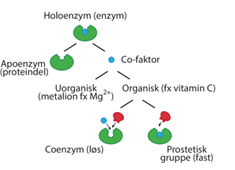
\includegraphics[width=0.8\textwidth]{figurs/enzym.png}
    \caption{Enzym}
    \label{fig:enzym}
\end{figure}
Enzymer er som sagt opbygget af proteiner, og måden disse proteiner bliver lavet er ved brug af en process der hedder det centrale dogme. Her bliver DNA lavet om til RNA som så bliver lavet om til protein. Det første trin i processen er transkription og det andet trin er translation. Under transkriptionen bliver DNA sekvensen analyseret og bliver omskrevet til hvad det vil svare til i en RNA sekvens ved brug af RNA-polymerase. Under translation bliver informationen på et mRNA-molekyle oversat til en rækkefølge af aminosyrer i et polypeptid ved brug af codonnets anticodon fra tRNA. Når der er dannet en lang kæde af aminosyrer bliver det så til et protein, som så kan bruges til at lave et enzym.
For at en reaktion kan foregå i kroppen skal to molekyler ramme hinanden hurtigt med en præcis vinke. Det lyder måske ikke så svært men man skal også huske at molekylerne ikke selv bestemmer hvordan de rejser rundt i blodet, da de ikke er levende. Dog kan det selvfølgeligt godt ske, dog er kravene til det meget svære at opnå uden ekstern hjælp. Det er der hvor enzymer kommer ind da de ”fanger” molekylerne og sikrer at de rammer hinanden med den rette orientering. Enzymet gør også så molekylerne ikke har brug for at have en høj nok bevægelsesenergi for at kunne reagere med hinanden og danne et nyt stof, uden et enzym ville man kunne øge bevægelsensenergien ved at øge temperaturen. Dog betyder det også at enzymer er meget specifikke og kan katalyserer en enkelt eller nogle få reaktioner. 
\begin{figure}
    \centering
    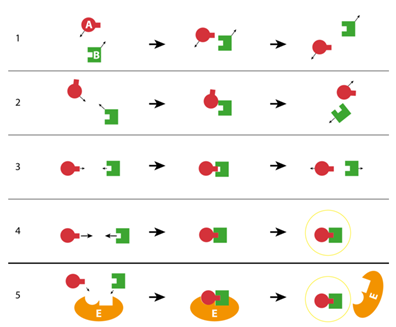
\includegraphics[width=0.8\textwidth]{figurs/enzym1.png}
    \caption{Enzym}
    \label{fig:enzym2}
\end{figure}
Det er faktisk ikke sindsygt svært at påvirke enzymer for enten det bedre eller det værre. Det kan man da enzymer virker bedst i specifikke miljøer og denaturer hvis miljøet er for ekstremt for dem. I øvelsen bromelin i ananas skulle vi klargøre en masse reagensglas med vand og opløst gelatine. I en af reagensglassene skulle vi tilsætte noget frisk ananasjuice fra en frisk presset ananas. Vi skulle også tilsætte konserveret ananassaft, ananasjuice og ananassaft fra dåse. I min gruppe puttede vi også saltsyre sammen med ananassaft for at se hvordan det daville påvirke gelatinens evne til at størkne. Formålet med øvelsen var at finde ud af hvornår et enzym, bromelin, ville hindre gelatine, som består af protein, i at størkne og danne gele. Vi gjorde det for at se om bromelin ville blive denatureret i forskellige miljø og hindre det i at virke. Her kunne vi tydeligt se hvor let det er at påvirke et enzym, for eksempel i reagensglasset med dåse ananas kunne vi se at der var der ingen reaktion mellem bromelinen og gelatinen. Det giver også god mening da dåsen formentligt er blevet varmebehandlet og derfor er bromelinen denatureret, da bromelinen er kommet i miljø der er alt for varmt og kommet over et point of no return. 
Der er mange konsekvenser ved mangel eller ændring af enzymer i en organisme, da hvis man mangler enzymer, kan nogle reaktioner ikke bliver katalyseret og derfor ikke finde sted i et stort nok omfang til at reaktionen er brugbar. En af de mere kendte sygdomme af mangel på et enzym er en tilstand kaldet laktoseintolerance. Her har personen ikke nok af enzymet laktase og vil derfor også have problemer med at nedbryde laktose. Ved ændring af enzymer i en organisme vil det samme nok også ske, dog kommer det selvfølgelig an på hvad det ændrer sig fra og hvad det ændrer sig til, dog er det nok typisk en dårlig ændring. Et eksempel på dette kan være at man har et enzym som katalyserer en livsnødvendig reaktion i kroppen, men så pludsligt af en ukendt årsag ændrer enzymet sig til noget andet som ikke kan katalyserer den samme reaktion. Det ville jo tydeligvis være meget dårligt da denne livsnødvendige reaktion ikke længere ville kunne foregå og organismen ville højest sandsynligt dø. 
